\section{Converged Graph Relational Optimization Framework}

\begin{figure}
    \centering
    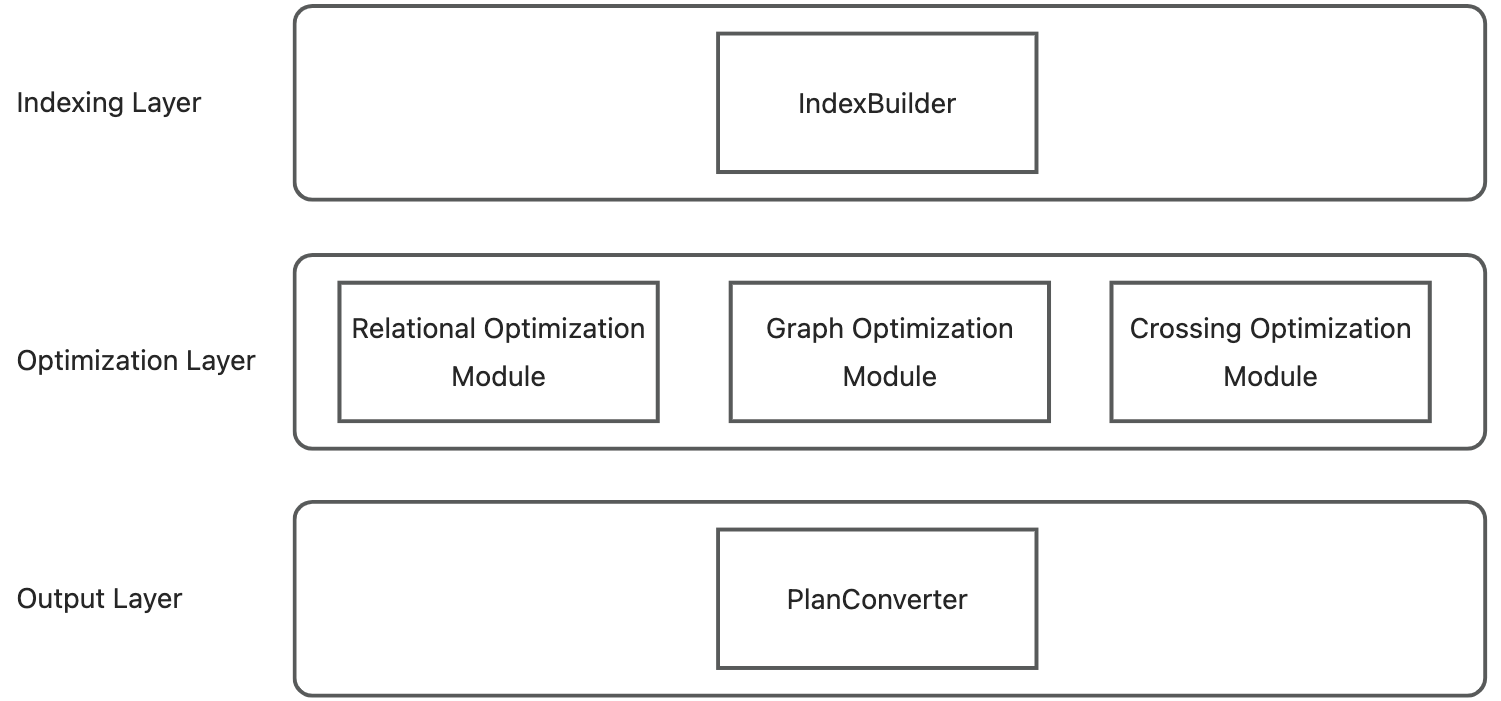
\includegraphics[width=\linewidth]{./figures/framework.png}
    \caption{Overview of the Converged Graph Relational Optimization Framwork.}
    \label{fig:framework-overview}
\end{figure}


The sketch of the converged graph relational optimization framework is shown in Fig.~\ref{fig:framework-overview}.
Specifically, given a SQL/PGQ query which contains graph queries, the query is firstly parsed and the corresponding logical plan is generated.
In such a SQL/PGQ query, it is straightforward to distinguish graph queries from relational queries, since the graph query are always marked with ``GRAPH\_TABLE (name, MATCH $\cdots$)''.

For each graph query, a graph logical plan is generated.
The operators that can be utilized in graph logical plans are those defined in graph relational algebra (introduced in Sec.~\ref{sec:preliminaries}).
Pleanse note that the output of a graph logical plan is a relational table.
Therefore, the graph logical plan can be considered to guide the process of retrieving data from a graph table, and the plan as a whole is a new implementation of the Scan operator, which is called ScanGraphTable.
The semantic of the ScanGraphTable operator is scanning a graph table obtained with graph queries.
Then, for the outer relational query, by representing graph queries with ScanGraphTable operators, the relational logical plan can be optimized by most relational optimizers such as Calcite.
Therefore, rich optimization strategies for relational databases can be applied.

In the process of optimization, the graph logical plans and the outer relational logical plan are optimized by the graph optimzation module and relaitonal optmization moduel, respectively.
The workflow of the converged graph relational optimization framework is illustrated with Fig.~\ref{fig:workflow}.
Firstly, graph queries are optimized with the graph optimization modules.
Both rule-based optimizations and cost-based optimizations are utilized.
Please note that during the process of optimizing the graph queries, the cardinalities of the outputs of the graph queries are estimated.
Then, in the following opimization for the relation query, the cardinalities of ScanGraphTable operators are obtained.
For the relaional optimization module, we propose two new rules specially for SQL/PGQ queries.
These rules push predicates in relational queries to graph queries to filter out the invalid elements early, and the details are introduced in Sec.~\ref{sec:optimizations}.
After the the relational query is optimized, it is tested whether the plan can be further optimized.
If the plan can still be optimized, then the graph opmization module and relational optimization module are applied again.
Otherwise, the optimal execution plan is obtained.


As different databases usually support different operators and their physical plans can be greatly varied, it is of critical importance for an optimization framework to be flexible.
Therefore, we implement a PlanConverter in the framework to ensure that the flexibility.
Given the generated optimal physical plan, the PlanConverter transforms the plan to an internal representation (e.g., substrait), and then the internal representation is transformed to the physical plan that can be executed by the target database.
Finally, the plan is executed and the query results are obtained.
The above process of query processing is illustrated with the following example.


\begin{figure}
    \centering
    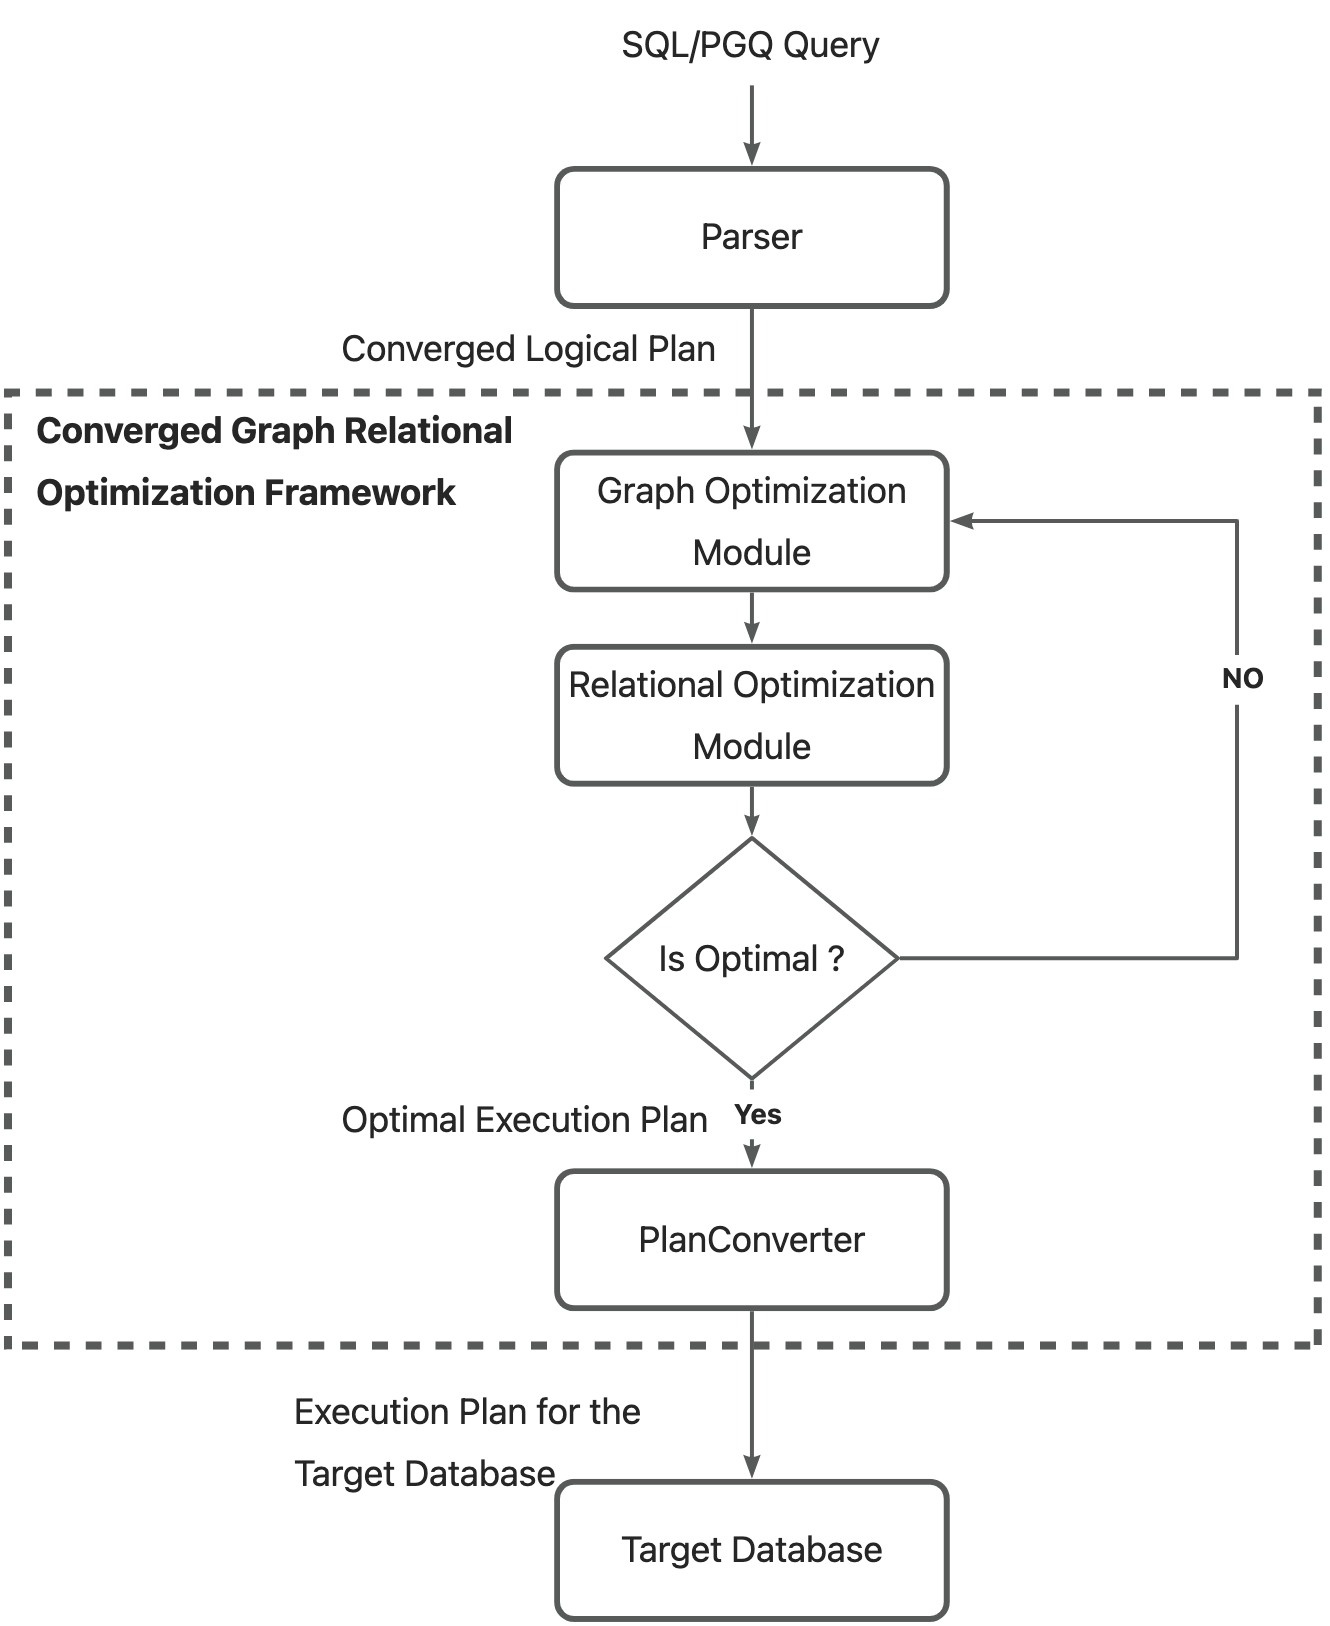
\includegraphics[width=.8\linewidth]{./figures/workflow.png}
    \caption{Workflow of the Converged Graph Relational Optimization Framework.}
    \label{fig:workflow}
\end{figure}


\begin{figure*}
    \centering
    \begin{subfigure}[b]{0.4\linewidth}
        \centering
        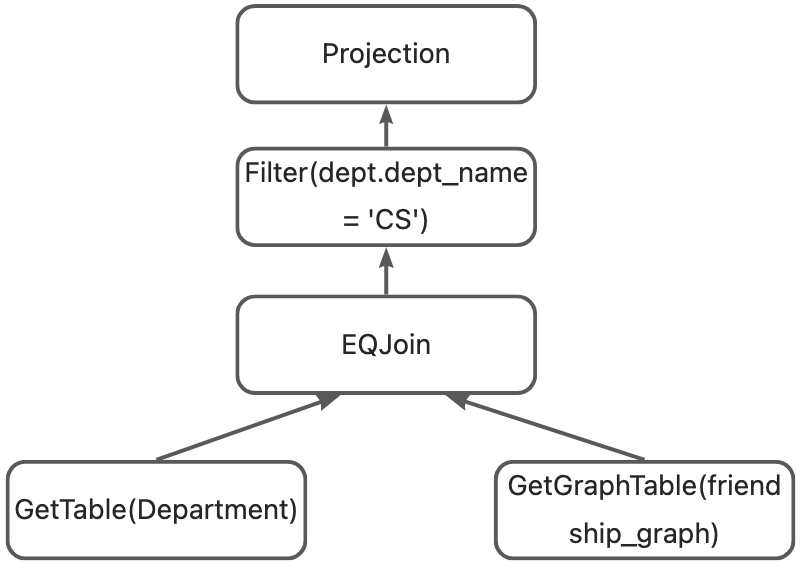
\includegraphics[width=\linewidth]{./figures/converged-logical-plan-relational.png}
        \caption{Relational Subplan of the Converged Logical Plan.}
        \label{fig:converged-logical-plan-relational}
    \end{subfigure}
    \begin{subfigure}[b]{0.4\linewidth}
        \centering
        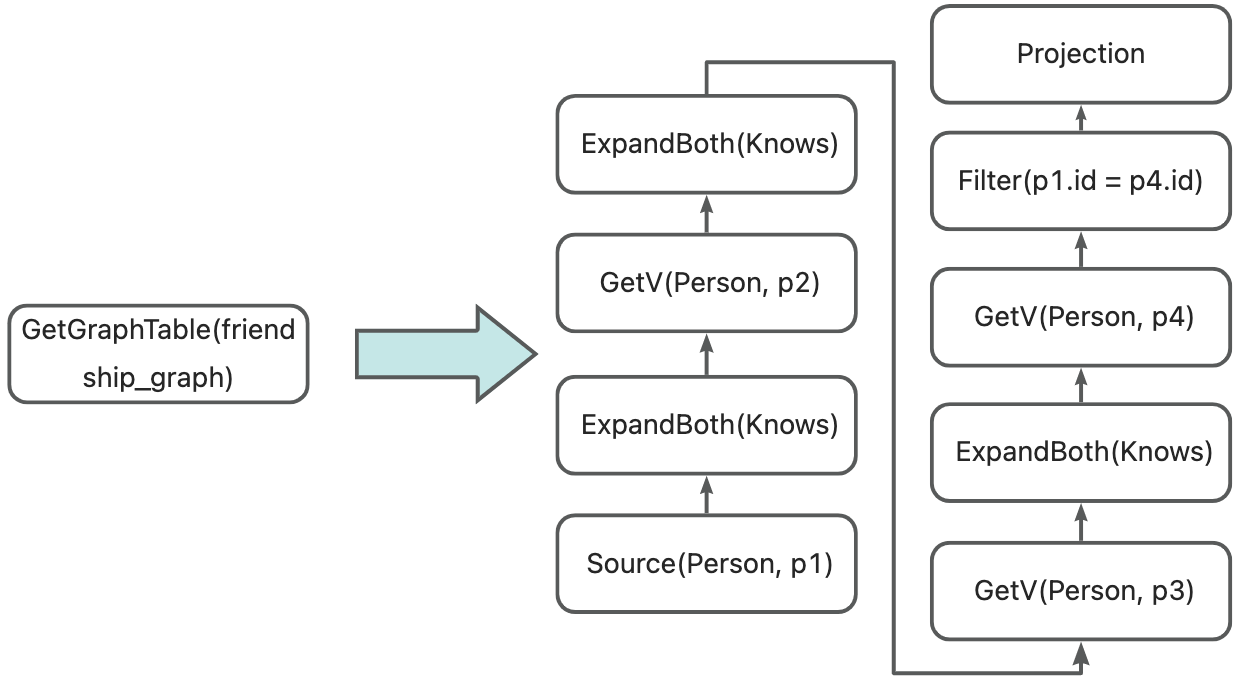
\includegraphics[width=\linewidth]{./figures/converged-logical-plan-graph.png}
        \caption{Graph Subplan of the Converged Logical Plan.}
        \label{fig:converged-logical-plan-graph}
    \end{subfigure}
    \begin{subfigure}[b]{0.4\linewidth}
        \centering
        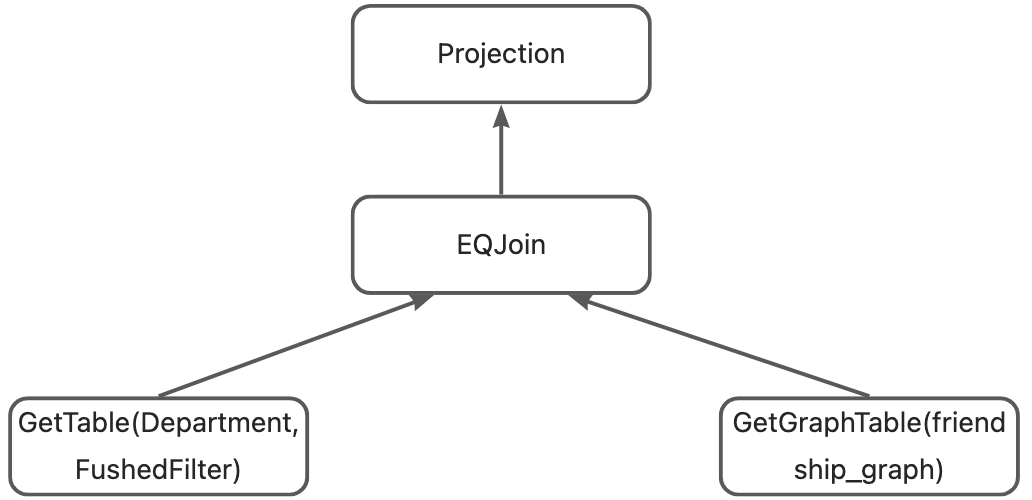
\includegraphics[width=\linewidth]{./figures/converged-logical-plan-relational-optimized.png}
        \caption{Relational Subplan after Optimization.}
        \label{fig:relational-plan-optimized}
    \end{subfigure}
    \begin{subfigure}[b]{0.4\linewidth}
        \centering
        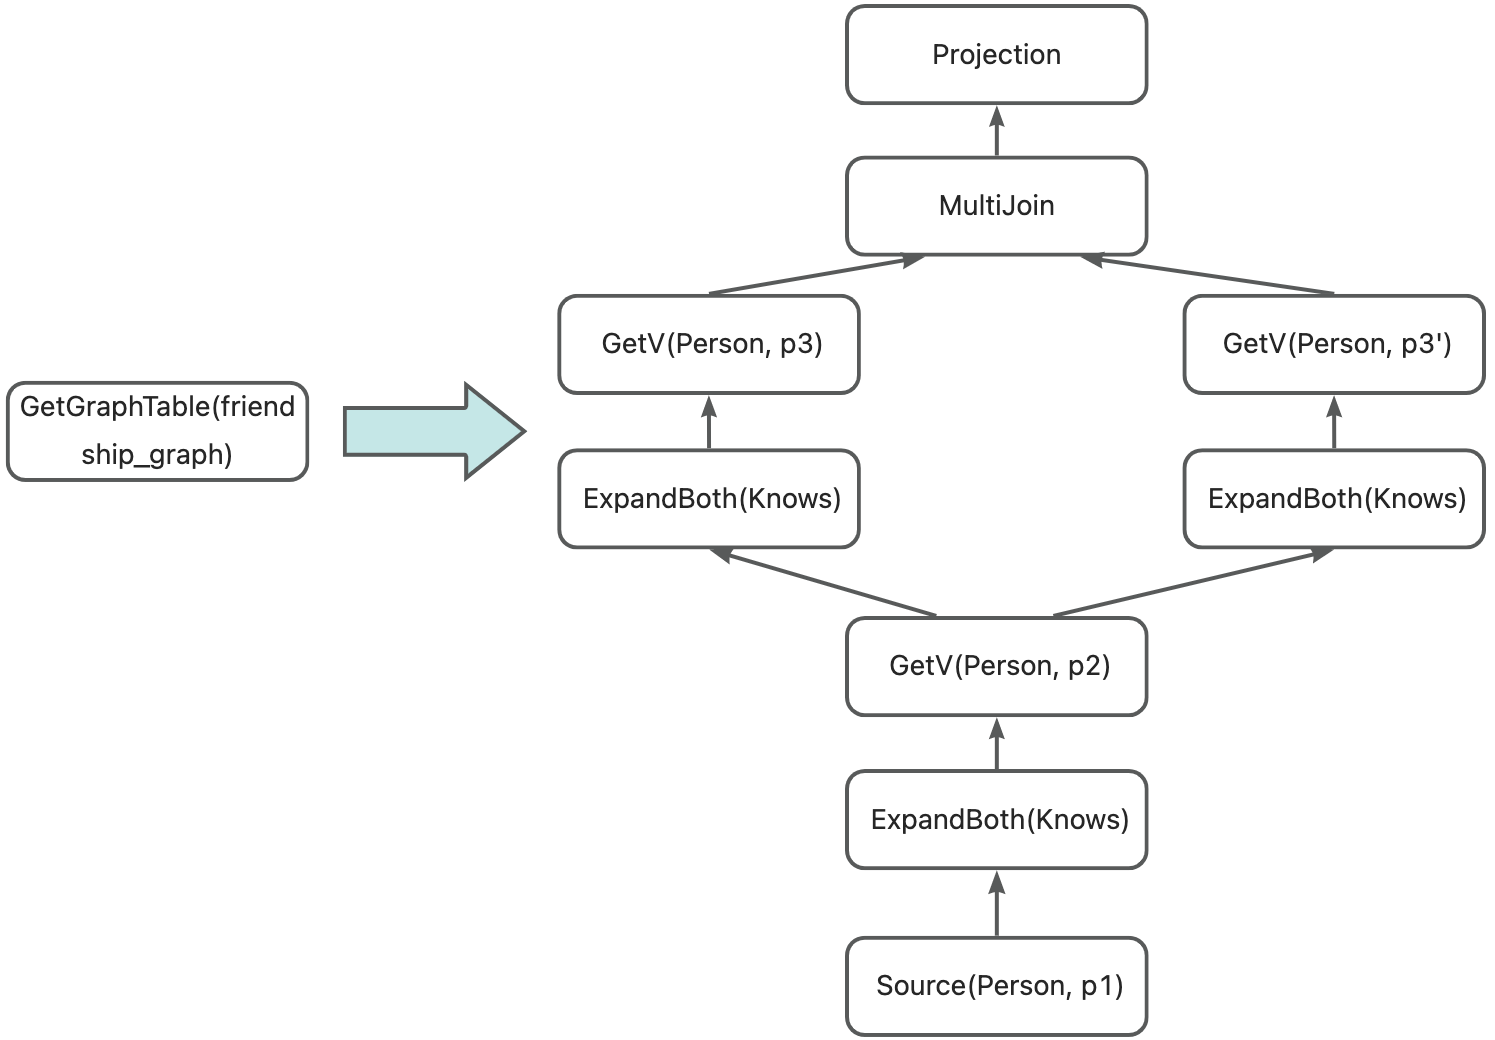
\includegraphics[width=\linewidth]{./figures/converged-logical-plan-graph-optimized.png}
        \caption{Graph Subplan after Optimization.}
        \label{fig:graph-plan-optimized}
    \end{subfigure}
    \begin{subfigure}[b]{0.4\linewidth}
        \centering
        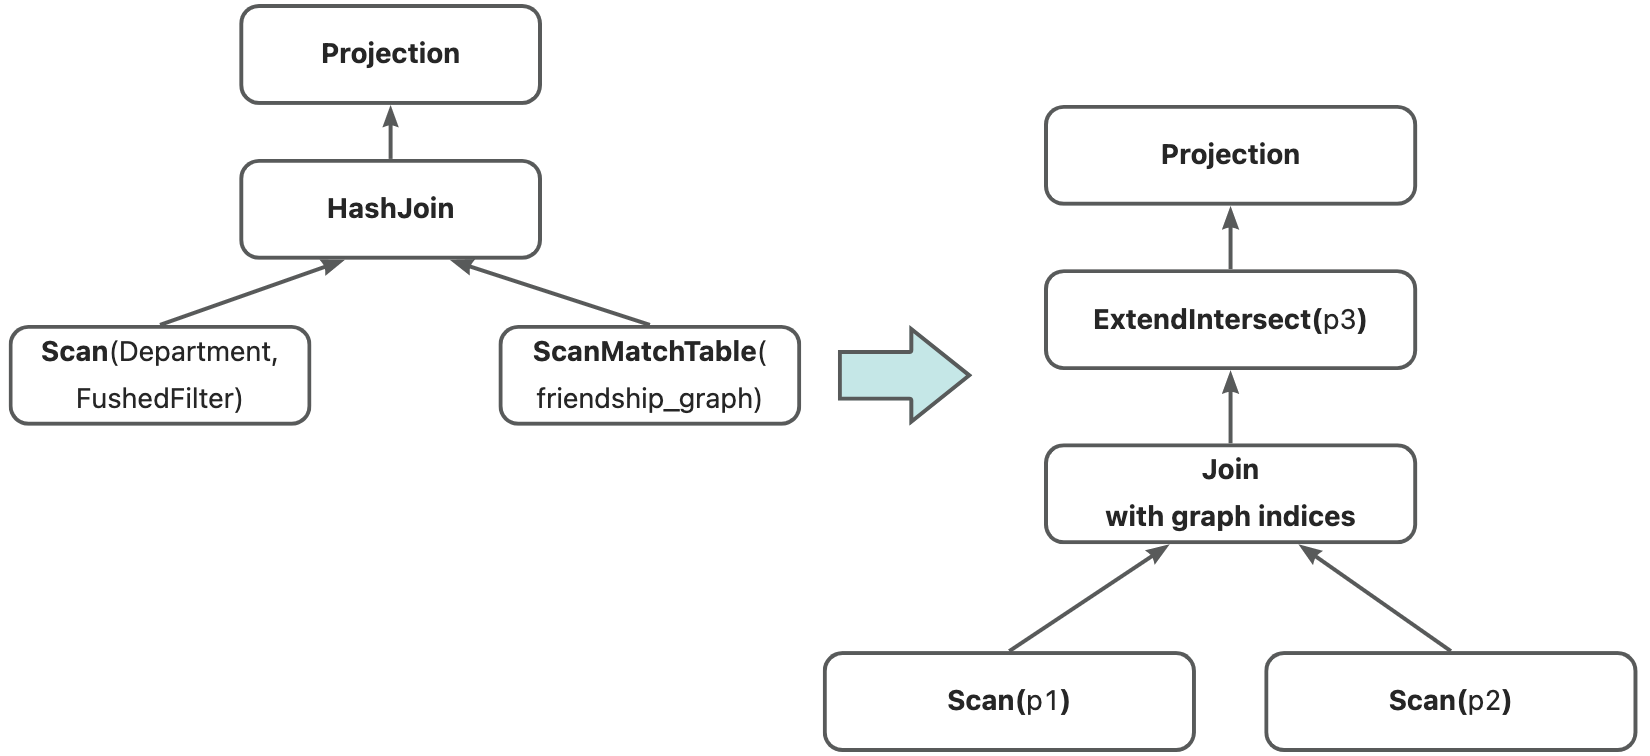
\includegraphics[width=\linewidth]{./figures/converged-physical-plan.png}
        \caption{Obtained Optimial Physical Plan.}
        \label{fig:physical-plan-optimized}
    \end{subfigure}
    \caption{An example of query opitmization.}
    \label{fig:query-grtree-example}
\end{figure*}


The above process of query processing is illustrated with the following example.

\begin{example}
    Given a relational database with tables as follows,
    \begin{equation*}
        \begin{split}
            & \textit{Person = (\underline{id}, name, dept\_id)} \\
            & \textit{Knows = (\underline{id1}, \underline{id2})} \\
            & \textit{Department = (\underline{dept\_id}, dept\_name)}, \\
        \end{split}
    \end{equation*}
    suppose we are going to find three persons satisfying: 
    (1) These three persons know each other;
    (2) At least two of them are from the department of computer science.
    The SQL/PGQ query for this task is shown in Example \ref{example:introduction:sqlpgq}.      

    There is one graph query for obtaining triangles of persons that know each other.
    Therefore, the converged logical plan consists of one relational subplan and one graph subplan.
    The algebra expression corresponding to this query is as follows:
    Firstly, to obtain the triangles, the graph relational algebra expression is
    \begin{equation*}
        \begin{split}
            G_{\triangle} = & \sigma_{p4.id = p1.id}(\updownarrow_{(p3)}^{(p4)}[:Knows]\updownarrow_{(p2)}^{(p3:Person)}[:Knows] \\
            & \updownarrow_{(p1)}^{(p2:Person)}[:Knows]\bigcirc_{(p1:Person)}).
        \end{split}
    \end{equation*}
    Then, to get the results of the graph query and formulate the results as a relational table, the algebra expression is 
    \begin{equation*}
        \begin{split}
            R_{graph} = & \pi_{p1.name\rightarrow pn1, p1.dept\_id \rightarrow dept1,p2.name\rightarrow pn2, p2.dept\_id \rightarrow dept2,} \\
            & _{p3.name\rightarrow pn3, p3.dept\_id \rightarrow dept3}(G_{\triangle}).
        \end{split}
    \end{equation*}
    Finally, to obtain the triangles of persons with at least two persons from the department of computer science, the relational algebra expression is
    \begin{equation*}
        \begin{split}
        \pi_{pn1, pn2, pn3}
        (& \sigma_{dept.dept\_name = `Computer Science'}( \\ 
        & dept \Join_{dept1=dept.dept\_id \land dept2=dept.dept\_id} R_{graph})).
        \end{split}
    \end{equation*}

    Based on the above algebra expressions, the corresponding converged logical plan is shown, and its relational and graph subplans are presented in Fig.~\ref{fig:converged-logical-plan-relational} and Fig.~\ref{fig:converged-logical-plan-graph}, respectively.
    
    Then, optimization modules in the optimization layer are applied to optimize the relational subplan and graph subplans.
    The optimized converged logical plan is shown in Fig.~\ref{fig:relational-plan-optimized} and Fig.~\ref{fig:graph-plan-optimized}.
    Moreover, the finally obtained optimal physical plan is shown in Fig.~\ref{fig:physical-plan-optimized}.
\end{example}

